\documentclass[a4paper,11pt]{article}
\usepackage[british]{babel}
\usepackage{color, colortbl}
\definecolor{Gray}{gray}{0.9}
%\usepackage{mathptmx}
\usepackage{mathpazo}
%\usepackage{palatcm}
\usepackage{tikz}
\usetikzlibrary{arrows}
\usetikzlibrary{positioning}
\usetikzlibrary{decorations.pathreplacing}
\usepackage[enabled,section]{easy-todo}

\author{Stefan de Konink & Joost Cassee}

\newcommand*{\bus}{
\includegraphics[scale=0.02]{img/bus}}
\newcommand*{\ferry}{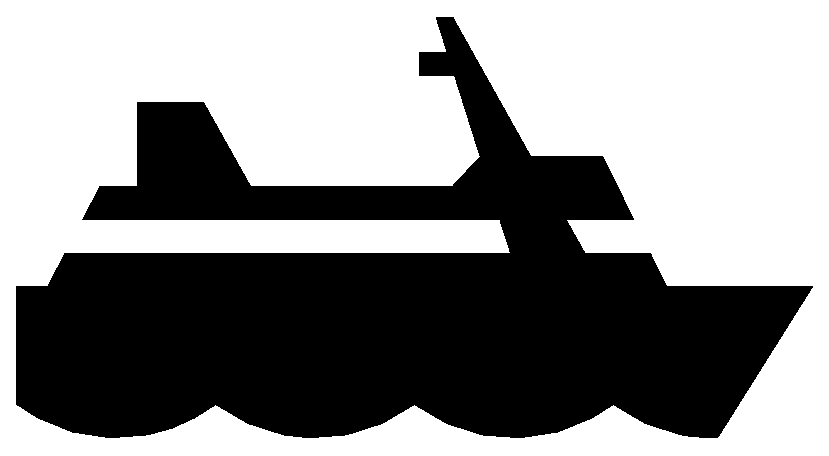
\includegraphics[scale=0.02]{img/ferry}}
\newcommand*{\train}{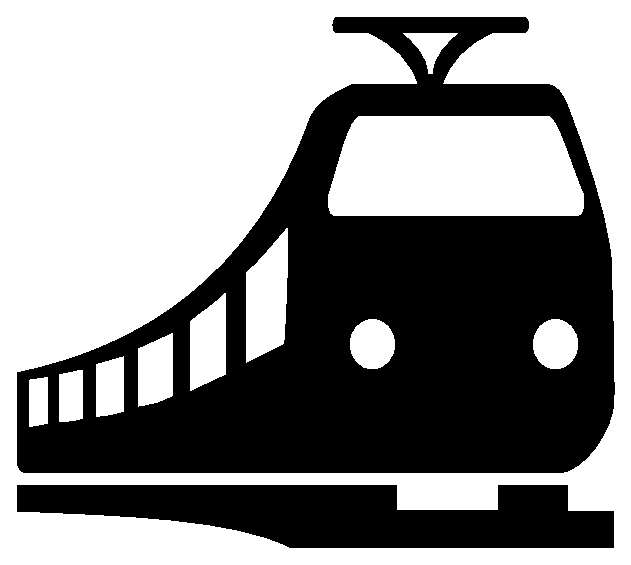
\includegraphics[scale=0.02]{img/train}}
\newcommand*{\walk}{
\includegraphics[scale=0.022]{img/walk}}
\renewcommand{\arraystretch}{1.2}

\begin{document}
\begin{enumerate}
\item \begin{enumerate}
\item \textit{All agencies and their published timetables including modalities bus, ferry, lightrail, metro, ferry and train given a departure time must be incorporatable in the journey planner.}
\subsubsection*{Network description and Timetable}
The network consists of three trips, each of a different modality to test if the journey planner is capable to traverse different modalities.
Each trip has a single linear timetable consisting of two stops.
All trips are planned sequentially.

\begin{figure}[h]
\vspace{1em}
\raggedleft
\begin{minipage}{305pt}
\resizebox{310pt}{!}{
\begin{tikzpicture}[->,>=stealth',shorten >=1pt,auto,node distance=3cm,
  thick,main node/.style={circle,fill=blue!20,draw,font=\sffamily\Large\bfseries}]

  \node[main node] (1) {1};
  \node[main node] (2) [right of=1] {2};
  \node[main node] (3) [right=1cm of 2] {3};
  \node[main node] (4) [right of=3] {4};
  \node[main node] (5) [right=1cm of 4] {5};
  \node[main node] (6) [right of=5] {6};
  \node (1a) [below=.2cm of 1] {00:01};
  \node (2a) [below=.2cm of 2] {00:02};
  \node (3a) [below=.2cm of 3] {00:03};
  \node (4a) [below=.2cm of 4] {00:04};
  \node (5a) [below=.2cm of 5] {00:05};
  \node (6a) [below=.2cm of 6] {00:06};

  \path[every node/.style={font=\sffamily\small}]
    (1) edge node {bus} (2)
    (3) edge node[yshift=-2pt] {ferry} (4)
    (5) edge node {train} (6);
\end{tikzpicture}
}
\end{minipage}
\label{fig:modalities_network}
\vspace{-2em}
\end{figure}

\subsubsection*{Synthetic Test}
\begin{enumerate}
\item \textbf{depart} at 00:00 from stop 1 heading to stop 6.
\end{enumerate}

\subsubsection*{Expected Result}
\begin{enumerate}
\item

{\scriptsize
\begin{tabular}{p{.75cm} | p{3.0cm} c p{3.0cm} | p{.75cm} }
\hline
\rowcolor{Gray}
Depart & From & & To & Arrive \\
\hline
00:01 & Stop 1 & \bus & Stop 2 & 00:02 \\
\hline
00:03 & Stop 3 & \ferry & Stop 4 & 00:04 \\
\hline
00:05 & Stop 5 & \train & Stop 6 & 00:06 \\
\hline
\end{tabular}
}

\end{enumerate}



\subsubsection*{Practical Test}
\begin{enumerate}
\item \textbf{depart} at 12:09pm from Amsterdam, Hagedoornweg heading to Amsterdam, Sloterdijk.
\end{enumerate}

\subsubsection*{Expected Result}
\begin{enumerate}
\item 
{\scriptsize
\begin{tabular}{p{.75cm} | p{3.0cm} c p{3.0cm} | p{.75cm} }
\hline
\rowcolor{Gray}
Depart & From & & To & Arrive \\
\hline
12:10 & Hagedoornweg & \bus & Buiksloterwegveer & 12:12 \\
\hline
  - & Buiksloterwegveer & \ferry & Amsterdam CS & - \\
\hline
12:27 & Amsterdam CS & \train & Amsterdam Sloterdijk & 12:33 \\
\hline
\end{tabular}
}
\end{enumerate}
\newpage
\item \textit{Under normal circumstances the journey planner should produce a valid travel advice within 5 seconds.}\\
\\
For each static test in this testset we will evaluate the responsetime of the journey planner.
The responses should always be less than 5 seconds.
\\
\item \textit{When calamities occur, the journey planner should produce a valid travel advice within 30 seconds.}\\
\\
For dynamic tests 3b, 3c, 3d, 3e, 3f, 3g and 3h we will evaluate the responsetime of the journey planner.
The responses in these test must always be given within 30 seconds.
\\

\item \textit{The journey planner must under any condition reply to a request.}\\
\\
Any request done in this testsuite must not abort the testsuite.
\\

\item \textit{The journey planner must guaranteed an uptime of 99.6\%.}\\
\\
At most 0.4\% of the request to the jourey planner, may fail.
\\

\item \textit{The planner reports in in all circumstances a valid traveladvice.}\\
\\
All tests must succesfully reply with a valid travel advice.
\\

\newpage

\item \textit{The journey planner is capable to optimise for a target arrival and departure time, and is able to plan on different operating days.}

\subsubsection*{Network description and Timetable}
The network consist of three trips, each of the same route and planned sequentially.
The timetable is valid for two operating days, and has an operating day without service in the middle.
We test if the journey planner is capable to select the expected trip based on arrive and a depart query for the operating day with service.
Additionally we check the result of the journey planner when a trip is requested on the operating day without service.

\begin{figure}[h]
\vspace{0.5em}
\raggedleft
\begin{minipage}{225pt}
\begin{tikzpicture}[->,>=stealth',shorten >=1pt,auto,node distance=3cm,
  thick,main node/.style={circle,fill=blue!20,draw,font=\sffamily\Large\bfseries}]

  \node[main node] (1) {1};
  \node[main node] (2) [right of=1] {2};

  \node (1a) [below=.2cm of 1] {00:01};
  \node (2a) [below=.2cm of 2] {00:02};
  \node (1b) [below=.1pt of 1a] {00:03};
  \node (2b) [below=.1pt of 2a] {00:04};
  \node (1c) [below=.1pt of 1b] {00:05};
  \node (2c) [below=.1pt of 2b] {00:06};

  \node (3a) [right of=2a] {2013-01-01, 1};
  \node (3b) [right of=2b] {2013-01-02, 0};
  \node (3c) [right of=2c] {2013-01-03, 1};

  \path[every node/.style={font=\sffamily\small}]
    (1) edge node {bus} (2);

\draw [-,decorate,decoration={brace,amplitude=10pt,mirror},yshift=0pt]
(1a.150) -- (1c.-150) node [black,midway,xshift=.1cm] {};

\draw [-,decorate,decoration={brace,amplitude=10pt},yshift=0pt]
(2a.30) -- (2c.-30) node [black,midway,xshift=.1cm] {};

\end{tikzpicture}
\end{minipage}
\label{fig:arrival_departure_network}
\vspace{-1.5em}
\end{figure}

\subsubsection*{Synthetic Tests}
\begin{enumerate}
\item on 2013-01-01 \textbf{depart} at 00:02 from stop 1 heading to stop 2.
\item from stop 1 heading stop 2 \textbf{arrive} at 00:03 on 2013-01-01.

\item on 2013-01-02 \textbf{depart} at 00:03 from stop 1 heading to stop 2.
\item from stop 1 heading stop 2 \textbf{arrive} at 00:04 on 2013-01-02.

\item on 2013-01-03 \textbf{depart} at 00:03 from stop 1 heading to stop 2.
\item from stop 1 heading stop 2 \textbf{arrive} at 00:04 on 2013-01-03.
\end{enumerate}


\subsubsection*{Expected Results}
\begin{enumerate}
\item
{\scriptsize
\begin{tabular}{p{1.4cm} | p{.75cm} | p{2.1cm} c p{2.1cm} | p{.75cm} }
\hline
\rowcolor{Gray}
Date & Depart & From & & To & Arrive \\
\hline
2013-01-01 & 00:03 & Stop 1 & \bus & Stop 2 & 00:04 \\
\hline
\end{tabular}
}

\item
{\scriptsize
\begin{tabular}{p{1.4cm} | p{.75cm} | p{2.1cm} c p{2.1cm} | p{.75cm} }
\hline
\rowcolor{Gray}
Date & Depart & From & & To & Arrive \\
\hline
2013-01-01 & 00:01 & Stop 1 & \bus & Stop 2 & 00:02 \\
\hline
\end{tabular}
}

\item
{\scriptsize
\begin{tabular}{p{1.4cm} | p{.75cm} | p{2.1cm} c p{2.1cm} | p{.75cm} }
\hline
\rowcolor{Gray}
Date & Depart & From & & To & Arrive \\
\hline
2013-01-03 & 00:01 & Stop 1 & \bus & Stop 2 & 00:02 \\
\hline
\end{tabular}
}

\item
{\scriptsize
\begin{tabular}{p{1.4cm} | p{.75cm} | p{2.1cm} c p{2.1cm} | p{.75cm} }
\hline
\rowcolor{Gray}
Date & Depart & From & & To & Arrive \\
\hline
2013-01-01 & 00:05 & Stop 1 & \bus & Stop 2 & 00:06 \\
\hline
\end{tabular}
}

\item
{\scriptsize
\begin{tabular}{p{1.4cm} | p{.75cm} | p{2.1cm} c p{2.1cm} | p{.75cm} }
\hline
\rowcolor{Gray}
Date & Depart & From & & To & Arrive \\
\hline
2013-01-03 & 00:03 & Stop 1 & \bus & Stop 2 & 00:04 \\
\hline
\end{tabular}
}

\item
{\scriptsize
\begin{tabular}{p{1.4cm} | p{.75cm} | p{2.1cm} c p{2.1cm} | p{.75cm} }
\hline
\rowcolor{Gray}
Date & Depart & From & & To & Arrive \\
\hline
2013-01-03 & 00:03 & Stop 1 & \bus & Stop 2 & 00:04 \\
\hline
\end{tabular}
}

\end{enumerate}
\end{enumerate}
\newpage

\item
\begin{enumerate}
\item \textit{The journey planner must optimise for shortest travel duration and include transfer times in its calculation.}
\subsubsection*{Network description and Timetable}
We describe a network consisting of two routes, calling at the same stops.
The routes have a different time demand type during the operating day, hence the travel duration between two stops is different during the day.

\begin{figure}[h]
\vspace{1em}
\raggedleft
\begin{minipage}{205pt}

\begin{tikzpicture}[->,>=stealth',shorten >=1pt,auto,node distance=3cm,
  thick,main node/.style={circle,fill=blue!20,draw,font=\sffamily\Large\bfseries}]

  \node[main node] (1) [] {1};
  \node[main node] (2) [right of=1] {2};
  \node[] (1a) [above=.2cm of 1] {00:01};
  \node[] (2a) [above=.2cm of 2] {00:02};
  \node[] (1z) [above=.1pt of 1a] {00:05};
  \node[] (2z) [above=.1pt of 2a] {00:07};
  \node[] (1b) [below=.2cm of 1] {00:01};
  \node[] (2b) [below=.2cm of 2] {00:03};
  \node[] (1c) [below=.1pt of 1b] {00:05};
  \node[] (2c) [below=.1pt of 2b] {00:06};

  \path[every node/.style={font=\sffamily\small}]
    (1) edge node {} (2)
    (1) edge [draw=blue,densely dotted,bend right=45] node {} (2);
\end{tikzpicture}
\end{minipage}
\label{fig:shortest_network}
\vspace{2em}
\end{figure}

The second network for this test consists of two routes which require some transfer time.
Due to the transfer time it is not possible to board the first and second trip between stop 5 and 6.
The only possible option is to board the first trip between stop 3 and 4, transfer and board the third trip between stop 5 and 6.

\begin{figure}[h]
\vspace{1em}
\raggedleft
\begin{minipage}{275pt}
\begin{tikzpicture}[->,>=stealth',shorten >=1pt,auto,node distance=3cm,
  thick,main node/.style={circle,fill=blue!20,draw,font=\sffamily\Large\bfseries}]

  \node[main node] (3) {3};
  \node[main node] (4) [right of=3] {4};
  \node[main node] (5) [right=1cm of 4] {5};
  \node[main node] (6) [right of=5] {6};
  \node (3a) [below=.2cm of 3] {00:01};
  \node (4a) [below=.2cm of 4] {00:02};
  \node (5a) [below=.2cm of 5] {00:02};
  \node (6a) [below=.2cm of 6] {00:03};

  \node (3b) [below=.1pt of 3a] {00:04};
  \node (4b) [below=.1pt of 4a] {00:05};
  \node (5b) [below=.1pt of 5a] {00:05};
  \node (6b) [below=.1pt of 6a] {00:06};

  \node (3c) [below=.1pt of 3b] {00:07};
  \node (4c) [below=.1pt of 4b] {00:08};
  \node (5c) [below=.1pt of 5b] {00:08};
  \node (6c) [below=.1pt of 6b] {00:09};

  \path[every node/.style={font=\sffamily\small}]
    (3) edge node[yshift=-2pt] {} (4)
    (5) edge[draw=blue,densely dotted] node {} (6);

  \path [loosely dashed] (4) edge node {\tiny 300s} (5);
\end{tikzpicture}
\end{minipage}
\label{fig:modalities_network}
\vspace{-0em}
\end{figure}

\subsubsection*{Synthetic Tests}
\begin{enumerate}
\item \textbf{depart} at 00:01 from stop 1 heading to stop 2.
\item \textbf{depart} at 00:03 from stop 1 heading to stop 2.
\item \textbf{depart} at 00:01 from stop 3 heading to stop 6.
\item \textbf{depart} at 00:02 from stop 3 heading to stop 6.
\item from stop 3 heading to stop 6 \textbf{arrive} at 00:09.
\end{enumerate}

\subsubsection*{Expected Results}
\begin{enumerate}
\item
{\scriptsize
\begin{tabular}{p{.75cm} | p{3.0cm} c p{3.0cm} | p{.75cm} }
\hline
\rowcolor{Gray}
Depart & From & & To & Arrive \\
\hline
00:01 & Stop 1 & \bus & Stop 2 & 00:02 \\
\hline
\end{tabular}
}
\item
{\scriptsize
\begin{tabular}{p{.75cm} | p{3.0cm} c p{3.0cm} | p{.75cm} }
\hline
\rowcolor{Gray}
Depart & From & & To & Arrive \\
\hline
00:05 & Stop 1 & \bus & Stop 2 & 00:06 \\
\hline
\end{tabular}
}
\item
{\scriptsize
\begin{tabular}{p{.75cm} | p{3.0cm} c p{3.0cm} | p{.75cm} }
\hline
\rowcolor{Gray}
Depart & From & & To & Arrive \\
\hline
00:01 & Stop 3 & \bus & Stop 4 & 00:02 \\
\hline
00:02 & Stop 4 & \walk & Stop 5 & 00:07 \\
\hline
00:08 & Stop 4 & \bus & Stop 6 & 00:09 \\
\hline
\end{tabular}
}
\item
{\scriptsize
\begin{tabular}{p{.75cm} | p{3.0cm} c p{3.0cm} | p{.75cm} }
\hline
\rowcolor{Gray}
Depart & From & & To & Arrive \\
\hline
00:01 & Stop 3 & \bus & Stop 4 & 00:02 \\
\hline
00:02 & Stop 4 & \walk & Stop 5 & 00:07 \\
\hline
00:08 & Stop 4 & \bus & Stop 6 & 00:09 \\
\hline
\end{tabular}
}
\item
{\scriptsize
\begin{tabular}{p{.75cm} | p{3.0cm} c p{3.0cm} | p{.75cm} }
\hline
\rowcolor{Gray}
Depart & From & & To & Arrive \\
\hline
00:01 & Stop 3 & \bus & Stop 4 & 00:02 \\
\hline
00:02 & Stop 4 & \walk & Stop 5 & 00:07 \\
\hline
00:08 & Stop 4 & \bus & Stop 6 & 00:09 \\
\hline
\end{tabular}
}
\end{enumerate}
\newpage

%%%%%%%%%%%%%%%%%%%

\item \textit{The journey planner should allow personalisation of the result prioritising vehicle attributes such as seats availability, (wheelchair) accessibility, toilets, WiFi, etc.}
\subsubsection*{Network description and Timetable}
The network consists of one route and two trips.
The trip attribute $x$ is available for the vehicle of the second trip.

\begin{figure}[h]
\vspace{1em}
\raggedleft
\begin{minipage}{205pt}
\begin{tikzpicture}[->,>=stealth',shorten >=1pt,auto,node distance=3cm,
  thick,main node/.style={circle,fill=blue!20,draw,font=\sffamily\Large\bfseries}]

  \node[main node] (1) [] {1};
  \node[main node] (2) [right of=1] {2};
  \node[] (1a) [above=.2cm of 1] {00:01};
  \node[] (1b) [below=.2cm of 1] {00:03};
  \node[] (2a) [above=.2cm of 2] {00:02};
  \node[] (2b) [below=.2cm of 2] {00:04};

  \path (1.15) edge node {$x=0$} (2.165);
  \path (1.-15) edge [draw=blue,densely dotted] node [yshift=-14pt,pos=0.5,style={font=\sffamily\small}] {$x=1$} (2.195);
\end{tikzpicture}
\end{minipage}
\label{fig:attributes_network}
\vspace{-2em}
\end{figure}

\subsubsection*{Synthetic Test}
\begin{enumerate}
\item \textbf{depart} at 00:01 from stop 1 heading to stop 2, wants $x = 1$.
\end{enumerate}

\subsubsection*{Expected Result}
\begin{enumerate}
\item
{\scriptsize
\begin{tabular}{p{.75cm} | p{3.0cm} c p{3.0cm} | p{.75cm} }
\hline
\rowcolor{Gray}
Depart & From & & To & Arrive \\
\hline
00:03 & Stop 1 & \bus & Stop 2 & 00:04 \\
\hline
\end{tabular}
}
\end{enumerate}
\newpage

%%%%%%%%%%%%%%%%%%%%%%

\item \textit{The journey planner allows to personalise for least transfers and preferred modalities.}

\subsubsection*{Network description and Timetable}
This network consist of three routes.
Both start points (stop 1 and 4) and end points (stop 3 and 5) are the same stop area.
The two train routes including the transfer at two is slightly faster than taking the bus.
The test will evaluate if the planner prioritises modaliy and least transfers over shortest arrival time.

\begin{figure}[h]
\vspace{1em}
\raggedleft
\begin{minipage}{245pt}
\begin{tikzpicture}[->,>=stealth',shorten >=1pt,auto,node distance=3cm,
  thick,main node/.style={circle,fill=blue!20,draw,font=\sffamily\Large\bfseries}]

  \node[main node] (1) [] {1};
  \node[main node] (4) [below=1cm of 1] {4};
  \node[main node] (2) [right of=1] {2};
  \node[main node] (3) [right of=2] {3};
  \node[main node] (5) [below=1cm of 3] {5};

  \node[] (1b) [below=.2cm of 1] {00:01};
  \node[] (2b) [below=.2cm of 2] {00:02};
  \node[] (2a) [above=.2cm of 2] {00:03};
  \node[] (3a) [above=.2cm of 3] {00:04};
  \node[] (3b) [below=.2cm of 4] {00:02};
  \node[] (5b) [below=.2cm of 5] {00:06};

  \path[every node/.style={font=\sffamily\small}]
    (1) edge node {train} (2)
    (2) edge [draw=blue,densely dotted] node {train} (3)
    (4) edge [draw=red,dashed] node {bus} (5);
\end{tikzpicture}
\end{minipage}
\label{fig:singlemodality_network}
\vspace{-2em}
\end{figure}

\subsubsection*{Synthetic Tests}
\begin{enumerate}
\item \textbf{depart} at 00:01 from stop 1 heading to stop 3.
\item \textbf{depart} at 00:01 from stop 1 heading to stop 3, prefer bus.
\item \textbf{depart} at 00:01 from stop 1 heading to stop 3, prefer least transfers.
\end{enumerate}

\subsubsection*{Expected Results}
\begin{enumerate}
\item
{\scriptsize
\begin{tabular}{p{.75cm} | p{3.0cm} c p{3.0cm} | p{.75cm} }
\hline
\rowcolor{Gray}
Depart & From & \hspace{0.4cm} & To & Arrive \\
\hline
00:01 & Stop 1 & \train & Stop 2 & 00:03 \\
\hline
00:03 & Stop 1 & \train & Stop 2 & 00:04 \\
\hline
\end{tabular}
}
\item
{\scriptsize
\begin{tabular}{p{.75cm} | p{3.0cm} c p{3.0cm} | p{.75cm} }
\hline
\rowcolor{Gray}
Depart & From & \hspace{0.4cm} & To & Arrive \\
\hline
00:01 & Stop 1 & \walk & Stop 4 & 00:02 \\
\hline
00:02 & Stop 4 & \bus & Stop 5 & 00:06 \\
\hline
00:06 & Stop 5 & \walk & Stop 3 & 00:07 \\
\hline
\end{tabular}
}
\item
{\scriptsize
\begin{tabular}{p{.75cm} | p{3.0cm} c p{3.0cm} | p{.75cm} }
\hline
\rowcolor{Gray}
Depart & From & \hspace{0.4cm} & To & Arrive \\
\hline
00:01 & Stop 1 & \walk & Stop 4 & 00:02 \\
\hline
00:02 & Stop 4 & \bus & Stop 5 & 00:06 \\
\hline
00:06 & Stop 5 & \walk & Stop 3 & 00:07 \\
\hline
\end{tabular}
}
\end{enumerate}
\newpage 

%%%%%%%%%%%%%%%%%%%%%%

\item \textit{The journey planner uses stop-to-stop transfers in its advice.}
\subsubsection*{Network description and Timetable}
Stop-to-Stop transfers can be found at stations and stopplaces.
Typically this means that there is should be time reserved to alight and board between a trip departing at the same stop place.
The dwell time for the transfer is defined, or can be reduced to zero if enough time is available to make the transfer.

\begin{figure}[h]
\vspace{1em}
\raggedleft
\begin{minipage}{265pt}
\begin{tikzpicture}[->,>=stealth',shorten >=1pt,auto,node distance=3cm,
  thick,main node/.style={circle,fill=blue!20,draw,font=\sffamily\Large\bfseries}]

  \node[main node] (3) {3};
  \node[main node] (1) [above left=1.5cm and 3cm of 3] {1};
  \node[main node] (2) [below left=1.5cm and 3cm of 3] {2};
  \node[main node] (4) [above right=1.5cm and 3cm of 3] {4};
  \node[main node] (5) [below right=1.5cm and 3cm of 3] {5};

  \node[] (1a)  [above=.2cm of 1] {00:01};
  \node[] (2b1) [below=.2cm of 2] {00:02};
  \node[] (2b2) [below=.6cm of 2] {00:06};
  \node[] (3a)  [above=.2cm of 3] {00:03};
  \node[] (3b1) [below=.2cm of 3] {00:03};
  \node[] (3b2) [below=.6cm of 3] {00:07};
  \node[] (4b1) [below=.2cm of 4] {00:04};
  \node[] (4b2) [below=.6cm of 4] {00:08};
  \node[] (5a)  [above=.2cm of 5] {00:05};

  \path[every node/.style={font=\sffamily\small}]
    (1) edge [draw=blue,densely dotted] node {} (3)
    (2) edge node {} (3)
    (3) edge node {} (4)
    (3) edge [draw=blue,densely dotted] node {} (5);

  \draw[very thick] (0,2)--(0,1.4);
  \node[] (dwell) [above=1.6cm of 3] {dwell time: 0s};
\end{tikzpicture}
\end{minipage}
\label{fig:singlemodality_network}
\vspace{-2em}
\end{figure}

\subsubsection*{Synthetic Tests}
\begin{enumerate}
\item \textbf{given} a default dwell time of 60 seconds and a specified dwell time of 0 seconds at stop 3, \textbf{depart} at 00:01 from stop 1 heading to stop 4.
\end{enumerate}

\subsubsection*{Expected Results}
\begin{enumerate}
\item
{\scriptsize
\begin{tabular}{p{.75cm} | p{3.0cm} c p{3.0cm} | p{.75cm} }
\hline
\rowcolor{Gray}
Depart & From & \hspace{0.4cm} & To & Arrive \\
\hline
00:01 & Stop 1 & \train & Stop 2 & 00:03 \\
\hline
00:03 & Stop 3 & \train & Stop 4 & 00:04 \\
\hline
\end{tabular}
}
\end{enumerate}
\newpage

%%%%%%%%%%%%%%%%%%%%%%%%%%%%%

\item \textit{The journey planner uses trip-to-trip transfers in its advice.}
\subsubsection*{Network description and Timetable}
Trip-to-trip transfers allow the definition of prefered transfers that may be garanteed by the operator.
In a dynamic scenario a trip-to-trip transfer is guaranteed as if the last arriving trip was in time, so commuters can make the transfer.
This has realtime prediction implications which may delay the waiting trip.

\begin{figure}[h]
\vspace{1em}
\raggedleft
\begin{minipage}{265pt}
\begin{tikzpicture}[->,>=stealth',shorten >=1pt,auto,node distance=3cm,
  thick,main node/.style={circle,fill=blue!20,draw,font=\sffamily\Large\bfseries}]

  \node[main node] (3) {3};
  \node[main node] (1) [above left of=3] {1};
  \node[main node] (2) [below left of=3] {2};
  \node[main node] (4) [right of=3] {4};
  \node[main node] (5) [above right of=4] {5};
  \node[main node] (6) [below right of=4] {6};

  \path[every node/.style={font=\sffamily\small}]
    (1) edge node {} (3)
    (2) edge [draw=blue,densely dotted] node {} (3)
    (4) edge node {} (5)
    (4) edge [draw=blue,densely dotted] node {} (6);

  \path (3.15) edge (4.165);
  \path (3.-15) edge [draw=blue,densely dotted] (4.195);

  \node[] (t1) [below=.4cm of 1] {trip 1};
  \node[] (t2) [above=.4cm of 2] {trip 2};

  \node[] (1a) [above=.2cm of 1] {00:01};
  \node[] (2b) [below=.2cm of 2] {00:02};
  \node[] (3a) [above=.2cm of 3] {00:02};
  \node[] (3b) [below=.2cm of 3] {00:03};
  \node[] (4a) [above=.2cm of 4] {00:03};
  \node[] (4b) [below=.2cm of 4] {00:04};
  \node[] (5a) [above=.2cm of 5] {00:04};
  \node[] (6b) [below=.2cm of 6] {00:05};
\end{tikzpicture}
\end{minipage}
\label{fig:triptotrip_network}
\vspace{0em}
\end{figure}

A secondary trip-to-trip transfer is based on blockcodes.
A blockcode is assigned to a vehicle which operates on a predefined sequential pattern of trips.
An earlier delay within the pattern must be propagated to later trips, but it also guarantees that alighting and boarding between the last stop of the current trip and the first stop of the next trip is not required.

\begin{figure}[h]
\vspace{1em}
\raggedleft
\begin{minipage}{250pt}
\begin{tikzpicture}[->,>=stealth',shorten >=1pt,auto,node distance=3cm,
  thick,main node/.style={circle,fill=blue!20,draw,font=\sffamily\Large\bfseries}]

  \node[main node] (7) [] {7};
  \node[main node] (8) [right of=7] {8};
  \node[main node] (9) [right of=8] {9};

  \path[every node/.style={font=\sffamily\small}]
    (7) edge node {$b=1, t=1$} (8)
    (8) edge [draw=blue,densely dotted] node {$b=1, t=2$} (9);
\end{tikzpicture}
\end{minipage}
\label{fig:blocktoblock_network}
\vspace{0em}
\end{figure}

\subsubsection*{Synthetic Tests}
\begin{enumerate}
\item \textbf{given} a \textit{preferred} transfer from trip 1 to trip 2 at stop 3, \textbf{depart} at 00:01 from stop 1 heading to stop 6.
\item \textbf{given} a \textit{preferred} transfer from trip 1 to trip 2 at stop 4, \textbf{depart} at 00:01 from stop 1 heading to stop 6.
\item \textbf{given} a \textit{unpreferred} transfer from trip 1 to trip 2 at stop 3, \textbf{depart} at 00:01 from stop 1 heading to stop 6.
\item \textbf{given} a \textit{unpreferred} transfer from trip 1 to trip 2 at stop 4, \textbf{depart} at 00:01 from stop 1 heading to stop 6.
\end{enumerate}

\todo{Add tests for blockcode trip-to-trip transfers.}

\subsubsection*{Expected Results}
\begin{enumerate}
\item
{\scriptsize
\begin{tabular}{p{.75cm} | p{3.0cm} c p{3.0cm} | p{.75cm} }
\hline
\rowcolor{Gray}
Depart & From & \hspace{0.4cm} & To & Arrive \\
\hline
00:01 & Stop 1 & \train & Stop 3 & 00:02 \\
\hline
00:03 & Stop 3 & \train & Stop 4 & 00:05 \\
\hline
00:04 & Stop 4 & \train & Stop 6 & 00:05 \\
\hline
\end{tabular}
}
\item
{\scriptsize
\begin{tabular}{p{.75cm} | p{3.0cm} c p{3.0cm} | p{.75cm} }
\hline
\rowcolor{Gray}
Depart & From & \hspace{0.4cm} & To & Arrive \\
\hline
00:01 & Stop 1 & \train & Stop 3 & 00:02 \\
\hline
00:02 & Stop 3 & \train & Stop 4 & 00:03 \\
\hline
00:04 & Stop 4 & \train & Stop 6 & 00:05 \\
\hline
\end{tabular}
}
\item
{\scriptsize
\begin{tabular}{p{.75cm} | p{3.0cm} c p{3.0cm} | p{.75cm} }
\hline
\rowcolor{Gray}
Depart & From & \hspace{0.4cm} & To & Arrive \\
\hline
00:01 & Stop 1 & \train & Stop 3 & 00:02 \\
\hline
00:02 & Stop 3 & \train & Stop 4 & 00:03 \\
\hline
00:04 & Stop 4 & \train & Stop 6 & 00:05 \\
\hline
\end{tabular}
}
\item
{\scriptsize
\begin{tabular}{p{.75cm} | p{3.0cm} c p{3.0cm} | p{.75cm} }
\hline
\rowcolor{Gray}
Depart & From & \hspace{0.4cm} & To & Arrive \\
\hline
00:01 & Stop 1 & \train & Stop 3 & 00:02 \\
\hline
00:03 & Stop 3 & \train & Stop 4 & 00:04 \\
\hline
00:04 & Stop 4 & \train & Stop 6 & 00:05 \\
\hline
\end{tabular}
}
\end{enumerate}

\todo{Explain why you have added the intermediate stops.}

\newpage

%%%%%%%%%

\item \textit{The journey planner is capable to produce a pre-trip advice (stop to stop) and an on-trip advice based on current location to the last stop.}

\subsubsection*{Network description and Timetable}
We define a network of three routes, an intercity route between two stations, passing by a third station in the middle.
A local train is calling at all three of the stations and operates in both directions.
The user queries at the edge of the network between the first and second stop, while being on the intercity train.

\begin{figure}[h]
\vspace{1em}
\raggedleft
\begin{minipage}{250pt}
\begin{tikzpicture}[->,>=stealth',shorten >=1pt,auto,node distance=3cm,
  thick,main node/.style={circle,fill=blue!20,draw,font=\sffamily\Large\bfseries}]

  \node[main node] (1) [] {1};
  \node[main node] (2) [right of=1] {2};
  \node[main node] (3) [right of=2] {3};

  \path[every node/.style={font=\sffamily\small}]
    (1.30) edge [bend left=10] node {} (3.-210)
    (1) edge [draw=blue,densely dotted] node {} (2)
    (2) edge [draw=blue,densely dotted] node {} (3)
    (3.210) edge [draw=blue,densely dotted] node {} (2.-30)
    (2.210) edge [draw=blue,densely dotted] node {} (1.-30)
    (2.210) edge [draw=blue,densely dotted] node {} (1.-30);

  \node[] (1a) [above=.2cm of 1] {00:01};
  \node[] (3a) [above=.2cm of 3] {00:04};

  \node[] (1b) [below=.2cm of 1] {00:01};
  \node[] (2b) [below=.2cm of 2] {00:03};
  \node[] (3b) [below=.2cm of 3] {00:05};

  \node[] (3b) [below=.1pt of 3b] {00:06};
  \node[] (2b) [below=.1pt of 2b] {00:09};
  \node[] (1b) [below=.1pt of 1b] {00:11};

\draw[very thick] (1.5,1)--(1.5,0.4);
\end{tikzpicture}
\end{minipage}
\label{fig:ontrip_network}
\vspace{0em}
\end{figure}

\subsubsection*{Synthetic Tests}
\begin{enumerate}
\item \textbf{depart} from trip 1 heading stop 2.
\end{enumerate}

\subsubsection*{Expected Results}
\begin{enumerate}
\item
{\scriptsize
\begin{tabular}{p{.75cm} | p{3.0cm} c p{3.0cm} | p{.75cm} }
\hline
\rowcolor{Gray}
Depart & From & \hspace{0.4cm} & To & Arrive \\
\hline
00:01 & Stop 1 & \train & Stop 3 & 00:04 \\
\hline
00:06 & Stop 3 & \train & Stop 2 & 00:09 \\
\hline
\end{tabular}
}
\end{enumerate}

\end{enumerate}
\newpage
%%%%%%%%%%%%%%%%%%%%%%%%%%%%%%%%%%%%%%%%%%%%%%%%%%%%%
\item
\begin{enumerate}

\item \textit{The journey planner is capable to process planned changes in the regular publications automatically.} \\
\\
The ability to automatic load KV1 files is guaranteed using this testset.\\

%%%%%%%%%%%%%%%

\item \textit{The journey planner is capable to process unplanned changes in the regular publications automatically.}

\subsubsection*{Network description and Timetable}
The network consists of two stops, with a ten minute interval service, we present two trips.
The first trip has an initial delay of 10 minutes, the second trip has an intial lag of one minute.
The test determines which trip is prefered.

\begin{figure}[h]
\vspace{1em}
\raggedleft
\begin{minipage}{285pt}
\begin{tikzpicture}[->,>=stealth',shorten >=1pt,auto,node distance=3cm,
  thick,main node/.style={circle,fill=blue!20,draw,font=\sffamily\Large\bfseries}]

  \node[main node] (1) [] {1};
  \node[main node] (2) [right of=1] {2};
  \node[] (1a) [above=.2cm of 1] {00:01};
  \node[] (1b) [below=.2cm of 1] {00:11};
  \node[] (2a) [above=.2cm of 2] {00:02};
  \node[] (2b) [below=.2cm of 2] {00:12};

  \node[] (6) [left=1cm of 1a] {\tiny KV6 delay: 600s};
  \node[] (17) [left=1cm of 1b] {\tiny KV17 lag: 60s};

  \path (1.15) edge node {} (2.165);
  \path (1.-15) edge [draw=blue,densely dotted] node [yshift=-14pt,pos=0.5,style={font=\sffamily\small}] {} (2.195);
\end{tikzpicture}
\end{minipage}
\label{fig:delay_network}
\vspace{-2em}
\end{figure}

\subsubsection*{Synthetic Tests}
\begin{enumerate}
\item \textbf{depart} at 00:01 from Stop 1 heading Stop 2.
\item \textbf{depart} at 00:11 from Stop 1 heading Stop 2.
\end{enumerate}

\subsubsection*{Expected Results}
\begin{enumerate}
\item
{\scriptsize
\begin{tabular}{p{.75cm} | p{3.0cm} c p{3.0cm} | p{.75cm} }
\hline
\rowcolor{Gray}
Depart & From & \hspace{0.4cm} & To & Arrive \\
\hline
00:01 +10m & Stop 1 & \bus & Stop 2 & 00:02 +10m \\
\hline
\end{tabular}
}
\item
{\scriptsize
\begin{tabular}{p{.75cm} | p{3.0cm} c p{3.0cm} | p{.75cm} }
\hline
\rowcolor{Gray}
Depart & From & \hspace{0.4cm} & To & Arrive \\
\hline
00:01 +10m & Stop 1 & \bus & Stop 2 & 00:02 +10m \\
\hline
\end{tabular}
}
\end{enumerate}
\newpage
%%%%%%%%%%%%%%%

\item \textit{The journey planner is capable use changes within the travel advice, which may lead to a different travice advice.}

\subsubsection*{Network description and Timetable}
The network consists of three stops and two trips.
The first trip punctuality changes in a punctuality, while the second trip is in time.

\begin{figure}[h]
\vspace{1em}
\raggedleft
\begin{minipage}{245pt}
\begin{tikzpicture}[->,>=stealth',shorten >=1pt,auto,node distance=3cm,
  thick,main node/.style={circle,fill=blue!20,draw,font=\sffamily\Large\bfseries}]

  \node[main node] (1) [] {1};
  \node[main node] (2) [right of=1] {2};
  \node[main node] (3) [right of=2] {3};
  \node[] (1a) [above=.2cm of 1] {00:01};
  \node[] (1b) [below=.2cm of 1] {00:04};
  \node[] (2a) [above=.2cm of 2] {00:02};
  \node[] (2b) [below=.2cm of 2] {00:05};
  \node[] (3a) [above=.2cm of 3] {00:03};
  \node[] (3b) [below=.2cm of 3] {00:06};

  \path (1.15) edge node {\tiny p = 120s} (2.165);
  \path (2.15) edge node {\tiny p = 60s} (3.165);
  \path (1.-15) edge [draw=blue,densely dotted] node [yshift=-14pt,pos=0.5,style={font=\sffamily\small}] {} (2.195);
  \path (2.-15) edge [draw=blue,densely dotted] node [yshift=-14pt,pos=0.5,style={font=\sffamily\small}] {} (3.195);
\end{tikzpicture}
\end{minipage}
\label{fig:delay_network}
\vspace{-2em}
\end{figure}

\subsubsection*{Synthetic Tests}
\begin{enumerate}
\item \textbf{depart} at 00:04 from Stop 2 heading Stop 3.
\end{enumerate}

\subsubsection*{Expected Results}
\begin{enumerate}
\item
{\scriptsize
\begin{tabular}{p{.75cm} | p{3.0cm} c p{3.0cm} | p{.75cm} }
\hline
\rowcolor{Gray}
Depart & From & \hspace{0.4cm} & To & Arrive \\
\hline
00:02 +2m & Stop 2 & \bus & Stop 3 & 00:03 \textbf{+2m} \\
\hline
\end{tabular}
}
\\
\tiny{\textit{Note: keep in mind, that while the punctuality may reduce after stop 2, it is not yet known to the journey planner, \\ the \textbf{+2m} in the table may be reduced by a natural decay of the journey planner, we assume naive propagation.}}
\end{enumerate}
\newpage


%%%%%%%%%%%%%%%

\item \textit{The journey planner is capable to exclude routes from travice advice.}

\subsubsection*{Network description and Timetable}
The network consists of two stops, and two routes.
The first route is the fastest but is excluded.

\begin{figure}[h]
\vspace{1em}
\raggedleft
\begin{minipage}{205pt}
\begin{tikzpicture}[->,>=stealth',shorten >=1pt,auto,node distance=3cm,
  thick,main node/.style={circle,fill=blue!20,draw,font=\sffamily\Large\bfseries}]

  \node[main node] (1) [] {1};
  \node[main node] (2) [right of=1] {2};
  \node[] (1a) [above=.2cm of 1] {00:01};
  \node[] (1b) [below=.2cm of 1] {00:01};
  \node[] (2a) [above=.2cm of 2] {00:02};
  \node[] (2b) [below=.2cm of 2] {00:03};

  \path (1.15) edge node {} (2.165);
  \path (1.-15) edge [draw=blue,densely dotted] node [yshift=-14pt,pos=0.5,style={font=\sffamily\small}] {} (2.195);
\end{tikzpicture}
\end{minipage}
\label{fig:delay_network}
\vspace{-2em}
\end{figure}

\subsubsection*{Synthetic Tests}
\begin{enumerate}
\item \textbf{depart} at 00:01 from Stop 1 heading Stop 2 exclude route 1.
\end{enumerate}

\subsubsection*{Expected Results}
\begin{enumerate}
\item
{\scriptsize
\begin{tabular}{p{.75cm} | p{3.0cm} c p{3.0cm} | p{.75cm} }
\hline
\rowcolor{Gray}
Depart & From & \hspace{0.4cm} & To & Arrive \\
\hline
00:01 & Stop 1 & \bus & Stop 2 & 00:03 \\
\hline
\end{tabular}
}
\end{enumerate}
\vspace{2em}


%%%%%%%%%%%%%%%

\item \textit{The journey planner is capable to exclude trips from travice advice.}

\subsubsection*{Network description and Timetable}
The network consists of two stops, and two routes.
The first trip is is canceled by KV17, therefore it cannot be planned.

\begin{figure}[h]
\vspace{1em}
\raggedleft
\begin{minipage}{255pt}
\begin{tikzpicture}[->,>=stealth',shorten >=1pt,auto,node distance=3cm,
  thick,main node/.style={circle,fill=blue!20,draw,font=\sffamily\Large\bfseries}]

  \node[main node] (1) [] {1};
  \node[main node] (2) [right of=1] {2};
  \node[] (1b) [below=.2cm of 1] {00:01};
  \node[] (1c) [below=.1pt of 1b] {00:03};
  \node[] (2b) [below=.2cm of 2] {00:02};
  \node[] (2c) [below=.1pt of 2b] {00:04};
  \node[] (17) [left=.2cm of 1b] {\tiny KV17 cancel};

  \path (1) edge node {} (2);
\end{tikzpicture}
\end{minipage}
\label{fig:delay_network}
\vspace{-2em}
\end{figure}

\subsubsection*{Synthetic Tests}
\begin{enumerate}
\item \textbf{depart} at 00:01 from Stop 1 heading Stop 2 exclude route 1.
\end{enumerate}

\subsubsection*{Expected Results}
\begin{enumerate}
\item
{\scriptsize
\begin{tabular}{p{.75cm} | p{3.0cm} c p{3.0cm} | p{.75cm} }
\hline
\rowcolor{Gray}
Depart & From & \hspace{0.4cm} & To & Arrive \\
\hline
00:03 & Stop 1 & \bus & Stop 2 & 00:04 \\
\hline
\end{tabular}
}
\end{enumerate}

\newpage

%%%%%%%%%%%%%%%

\item \textit{The journey planner is capable to exclude stop places from travice advice.}

\subsubsection*{Network description and Timetable}
The network consists of four stops, and two routes.
The first route travels via the north, the second via the south.
The we do not want to pass through the North station.

\begin{figure}[h]
\vspace{1em}
\raggedleft
\begin{minipage}{225pt}
\begin{tikzpicture}[->,>=stealth',shorten >=1pt,auto,node distance=3cm,
  thick,main node/.style={circle,fill=blue!20,draw,font=\sffamily\Large\bfseries}]

  \node[main node] (1) [] {1};
  \node[main node] (2) [above right of=1] {2};
  \node[main node] (3) [below right of=2] {3};
  \node[main node] (4) [below right of=1] {4};

  \node[] (1a) [above=.2cm of 1] {00:01};
  \node[] (2a) [above=.2cm of 2] {00:02};
  \node[] (3a) [above=.2cm of 3] {00:03};
  \node[] (1b) [below=.2cm of 1] {00:01};
  \node[] (4b) [below=.2cm of 4] {00:02};
  \node[] (3b) [below=.2cm of 3] {00:04};

  \path[every node/.style={font=\sffamily\small}]
    (1) edge node {} (2)
    (2) edge node {} (3)
    (1) edge[draw=blue,densely dotted] node {} (4)
    (4) edge[draw=blue,densely dotted] node {} (3);

\end{tikzpicture}
\end{minipage}
\label{fig:delay_network}
\vspace{-2em}
\end{figure}

\subsubsection*{Synthetic Tests}
\begin{enumerate}
\item \textbf{depart} at 00:01 from Stop 1 heading Stop 3 exclude Stop 2.
\end{enumerate}

\subsubsection*{Expected Results}
\begin{enumerate}
\item
{\scriptsize
\begin{tabular}{p{.75cm} | p{3.0cm} c p{3.0cm} | p{.75cm} }
\hline
\rowcolor{Gray}
Depart & From & \hspace{0.4cm} & To & Arrive \\
\hline
00:01 & Stop 1 (via Stop 4) & \train & Stop 3 & 00:04 \\
\hline
\end{tabular}
}
\end{enumerate}

\newpage

%%%%%%%%%%%%%%%

\item \textit{The journey planner is capable to exclude stops from travice advice.}

\subsubsection*{Network description and Timetable}
In normal trip planning the planner would choose a place to alight and board trips based on preference of the operator (trip-to-trip), or an algorithm choose.
Especially at night not all stops might qualify to wait a bit for the next trip.
We exclude stops we do not want to alight and/or board from and allow this dynamic unpreferred transfer.

\begin{figure}[h]
\vspace{1em}
\raggedleft
\begin{minipage}{265pt}
\begin{tikzpicture}[->,>=stealth',shorten >=1pt,auto,node distance=3cm,
  thick,main node/.style={circle,fill=blue!20,draw,font=\sffamily\Large\bfseries}]

  \node[main node] (3) {3};
  \node[main node] (1) [above left of=3] {1};
  \node[main node] (2) [below left of=3] {2};
  \node[main node] (4) [right of=3] {4};
  \node[main node] (5) [above right of=4] {5};
  \node[main node] (6) [below right of=4] {6};

  \path[every node/.style={font=\sffamily\small}]
    (1) edge node {} (3)
    (2) edge [draw=blue,densely dotted] node {} (3)
    (4) edge node {} (5)
    (4) edge [draw=blue,densely dotted] node {} (6);

  \path (3.15) edge (4.165);
  \path (3.-15) edge [draw=blue,densely dotted] (4.195);

  \node[] (t1) [below=.4cm of 1] {trip 1};
  \node[] (t2) [above=.4cm of 2] {trip 2};

  \node[] (1a) [above=.2cm of 1] {00:01};
  \node[] (2b) [below=.2cm of 2] {00:02};
  \node[] (3a) [above=.2cm of 3] {00:02};
  \node[] (3b) [below=.2cm of 3] {00:03};
  \node[] (4a) [above=.2cm of 4] {00:03};
  \node[] (4b) [below=.2cm of 4] {00:04};
  \node[] (5a) [above=.2cm of 5] {00:04};
  \node[] (6b) [below=.2cm of 6] {00:05};
\end{tikzpicture}
\end{minipage}
\label{fig:triptotrip_network}
\vspace{0em}
\end{figure}

\subsubsection*{Synthetic Tests}
\begin{enumerate}
\item \textbf{given} a \textit{unpreferred} transfer from trip 1 to trip 2 at stop 3, \textbf{depart} at 00:01 from stop 1 heading to stop 6.
\item \textbf{given} a \textit{unpreferred} transfer from trip 1 to trip 2 at stop 4, \textbf{depart} at 00:01 from stop 1 heading to stop 6.
\end{enumerate}

\subsubsection*{Expected Results}
\begin{enumerate}
\item
{\scriptsize
\begin{tabular}{p{.75cm} | p{3.0cm} c p{3.0cm} | p{.75cm} }
\hline
\rowcolor{Gray}
Depart & From & \hspace{0.4cm} & To & Arrive \\
\hline
00:01 & Stop 1 & \train & Stop 4 & 00:03 \\
\hline
00:04 & Stop 4 & \train & Stop 6 & 00:05 \\
\hline
\end{tabular}
}
\item
{\scriptsize
\begin{tabular}{p{.75cm} | p{3.0cm} c p{3.0cm} | p{.75cm} }
\hline
\rowcolor{Gray}
Depart & From & \hspace{0.4cm} & To & Arrive \\
\hline
00:01 & Stop 1 & \train & Stop 3 & 00:02 \\
\hline
00:03 & Stop 3 & \train & Stop 6 & 00:05 \\
\hline
\end{tabular}
}
\end{enumerate}
\newpage

%%%%%%%%%%%%%%%

\item \textit{The journey planner must produce a valid travel advice when dynamic information is provided.
It must arrive at the best departure stop given the shortest total travel time.}

%%%%%%%%%%%%%%%

\item \textit{The journey planner should show if the planner incorporated dynamic information regarding calamities in the travel advice.}

%%%%%%%%%%%%%%%

\end{enumerate}

%%%%%%%%%%%%%%%%%%%%%%%%%%%%%%%%%%%%%%%%%%%%%%%%%%%%%
\item
\begin{enumerate}

\item \textit{The journey planner is aware of a punctuality change at the upcoming stop. Based on the provided punctuality it can predict the upcoming arrival and departure times.}

%%%%%%%%%%%%%%%

\item \textit{The journey planner is aware of the current timetable, timingstops and mutations on the operational process.}

%%%%%%%%%%%%%%%

\item \textit{The journey planner is aware of delays at the first vehicle in a sequence and is able to propagate it to latter vehicles with respect to future transfers. The travel advice results in an alternative using all available dynamic information in the journey planner.}

%%%%%%%%%%%%%%%

\item \textit{The journey planner is aware of delays in the previous trips, and suggests these delayed connections to give a shorter total transit time.}


\end{enumerate}


\end{enumerate}










\listoftodos

\end{document}
